
\documentclass{article}
\usepackage{amsmath, amssymb, bm}
\usepackage{geometry}
\usepackage{tikz}
\usepackage{pgfplots}
\usetikzlibrary{arrows.meta, decorations.markings}
\geometry{margin=1in}

\begin{document}

\section*{Degeneracy and Dual Uniqueness: Board Presentation with Diagram}

\textbf{Primal Linear Program (General Form):}
\[
\min \; c^T x \quad \text{subject to} \quad A x = b, \quad x \geq 0
\]

Assume:
\begin{itemize}
    \item \( x^* \) is a \textbf{non-degenerate basic feasible solution (BFS)},
    \item Let \( A = [A_B \;|\; A_N] \) be the partition into basic and non-basic columns,
    \item At a BFS: \( x_N = 0 \), and \( A_B \) is square and full rank,
    \item So: \( A_B x_B = b \Rightarrow x_B = A_B^{-1} b \)
\end{itemize}

\vspace{1em}

\textbf{Dual Linear Program:}
\[
\max \; b^T p \quad \text{subject to} \quad A^T p \leq c
\]

\[
A^T p =
\begin{bmatrix}
A_B^T \\
A_N^T
\end{bmatrix}
p
\leq
\begin{bmatrix}
c_B \\
c_N
\end{bmatrix}
\]

\textbf{Complementary Slackness:}
\begin{itemize}
    \item For active constraints (basic vars): \( x_B > 0 \Rightarrow A_B^T p^* = c_B \)
    \item Since \( A_B^T \) is invertible, this system has a \textbf{unique solution}:
    \[
    p^* = (A_B^T)^{-1} c_B
    \]
    \item For inactive constraints: \( x_N = 0 \Rightarrow p_N^* = 0 \)
\end{itemize}

\vspace{1em}

\textbf{Conclusion:} The complementary slackness conditions yield a full-rank square system that uniquely determines the dual solution when the primal is non-degenerate.

\vspace{2em}

\textbf{Geometric Illustration of Non-Degenerate BFS and Dual Uniqueness:}

\begin{center}
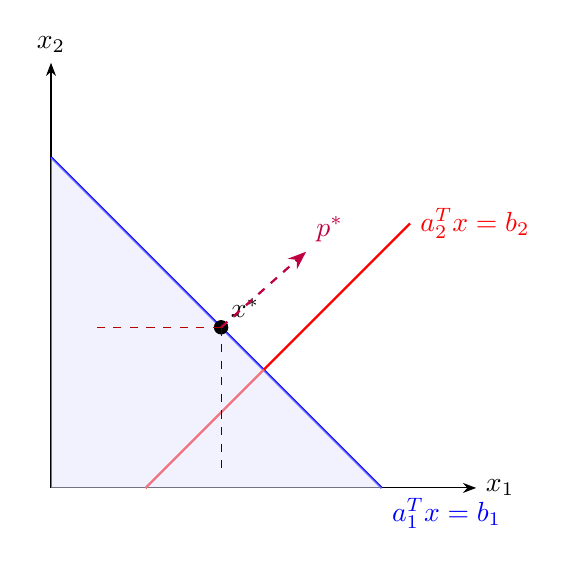
\begin{tikzpicture}[scale=1.2, >=Stealth]

% Axes
\draw[->] (0,0) -- (4.5,0) node[right] {$x_1$};
\draw[->] (0,0) -- (0,4.5) node[above] {$x_2$};

% Constraints (lines)
\draw[thick, blue] (0,3.5) -- (3.5,0) node[below right] {$a_1^T x = b_1$};
\draw[thick, red] (1,0) -- (3.8,2.8) node[right] {$a_2^T x = b_2$};

% Feasible region (shaded)
\fill[blue!10, opacity=0.5] (0,0) -- (0,3.5) -- (1.8,1.7) -- (3.5,0) -- cycle;

% Intersection point
\filldraw[black] (1.8,1.7) circle (2pt) node[above right] {$x^*$};

% Basis directions
\draw[dashed, blue!70!black] (1.8,1.7) -- (1.8,0.2);
\draw[dashed, red!70!black] (1.8,1.7) -- (0.4,1.7);

% Dual direction
\draw[->, thick, purple, dashed] (1.8,1.7) -- (2.7,2.5) node[above right] {$p^*$};

\end{tikzpicture}
\end{center}

\end{document}